\documentclass{beamer}

\usefonttheme{professionalfonts} % using non standard fonts for beamer
\usefonttheme{serif} % default family is serif

\usepackage{hyperref}

%\usepackage{minted}

\usepackage{animate}

\usepackage{graphicx}

\def\Put(#1,#2)#3{\leavevmode\makebox(0,0){\put(#1,#2){#3}}}

\usepackage{color}

\usepackage{tikz}

\usepackage{amssymb}
\usepackage{amsthm}

\usepackage{enumerate}

\usepackage{subcaption}

\newcommand\blfootnote[1]{%

  \begingroup

  \renewcommand\thefootnote{}\footnote{#1}%

  \addtocounter{footnote}{-1}%

  \endgroup

}

\makeatletter

%%%%%%%%%%%%%%%%%%%%%%%%%%%%%% Textclass specific LaTeX commands.

 % this default might be overridden by plain title style

 \newcommand\makebeamertitle{\frame{\maketitle}}%

 % (ERT) argument for the TOC

 \AtBeginDocument{%

   \let\origtableofcontents=\tableofcontents

   \def\tableofcontents{\@ifnextchar[{\origtableofcontents}{\gobbletableofcontents}}

   \def\gobbletableofcontents#1{\origtableofcontents}

 }

%%%%%%%%%%%%%%%%%%%%%%%%%%%%%% User specified LaTeX commands.

\usetheme{Malmoe}

% or ...

\useoutertheme{infolines}

\addtobeamertemplate{headline}{}{\vskip2pt}

\setbeamertemplate{theorems}[numbered]

\theoremstyle{definition}
\newtheorem{defn}{Definition}[section]

\setbeamercovered{transparent}

% or whatever (possibly just delete it)

\makeatother

\begin{document}
\title[Discussion 9]{CS/MATH 111, Discrete Structures - Fall 2018. \\ Discussion 9 - Graphs}
\author[CS111]{Andres, Sara, Elena}
\institute[Fall'18]{University of California, Riverside}
\makebeamertitle
\newif\iflattersubsect

\AtBeginSection[] {
    \begin{frame}<beamer>
    \frametitle{Outline} 
    \tableofcontents[currentsection]  
    \end{frame}
    \lattersubsectfalse
}

\AtBeginSubsection[] {
    \begin{frame}<beamer>
    \frametitle{Outline} 
    \tableofcontents[currentsubsection]  
    \end{frame}
}

\section{Bipartite graph}

\begin{frame}{Bipartite graph}
    \begin{itemize}
        \item A bipartite graph, also called a bigraph, is a set of graph vertices decomposed into two disjoint sets such that no two graph vertices within the same set are adjacent.
        \item Bipartite graphs are equivalent to two-colorable graphs. 
        \item All acyclic graphs are bipartite. 
        \item A cyclic graph is bipartite iff all its cycles are of even length
    \end{itemize}
\end{frame}

\begin{frame}{Bipartite graph}
    \centering \includegraphics[width=.7\linewidth]{p5.png}
\end{frame}

\section{Perfect matching}

\begin{frame}{Perfect matching}
A perfect matching of a graph is a matching (i.e., an independent edge set) in which every vertex of the graph is incident to exactly one edge of the matching. 
\\A perfect matching is therefore a matching containing $\frac{n}{2}$ edges (the largest possible), meaning perfect matchings are only possible on graphs with an even number of vertices.
\end{frame}

\begin{frame}{Perfect matching}
 Hall’s Theorem: Let G = (X,Y ) be a bipartite graph. Then X has a perfect macthing into Y if and only if for all $T \subseteq X$, the inequality $|T| \leq |N(T)|$ holds. Where N(T) is the set of all neighbors of the vertices in T. In other words, $y \in  Y$ is an element of N(T) if and only if there is a vertex $x \in  T$ so that xy is an edge.
\end{frame}

\begin{frame}{Perfect matching}
    \begin{flushleft}
        You are given two bipartite graph G and H below. For each graph determine whether it has a perfect matching. Justify your answer, either by listing the edges that are in the matching or use Hall's Theorem to show that the graph does not have a perfect matching.
    \end{flushleft}
    \centering \includegraphics[width=.7\linewidth]{p6.jpg}
\end{frame}

\begin{frame}{Perfect matching}
    \centering \includegraphics[width=.7\linewidth]{p7.png}
\end{frame}

\section{Trees}

\begin{frame}{Trees}
    \begin{lemma}
        It T is a tree, and has n vertices, then its number of edges is $m = n - 1$.
    \end{lemma}
\end{frame}

\begin{frame}{Proof (by induction)}
    \begin{enumerate}
        \item Basis step: 
        \begin{itemize}
            \item When $n = 1$, a tree with $n = 1$ vertex has no edges.  Indeed, $n -1 = 0$.
        \end{itemize}
        \item Assumption step:
        \begin{itemize}
            \item Let's assume that every tree with $k$ vertices has $k - 1$ edges, where $k$ is a positive integer.
        \end{itemize}
    \end{enumerate}
\end{frame}

\begin{frame}{Proof (cont.)}
    \begin{enumerate}[3]
        \item Inductive step: 
        \begin{itemize}
            \item Suppose that a tree $T$ has $k + 1$ vertices and that $v$ is a leaf\footnote{{\tiny It must exist because the tree is finite}} of $T$.  Let $w$ be the parent of $v$. 
            \item Remove $v$ from $T$ and the edge connecting $w$ to $v$. It produces a tree $T^\prime$ with $k$ vertices\footnote{ {\tiny $T^\prime$is still connected and has no simple circuits.}}. 
            \item By the assumption hypothesis, $T^\prime$ has $k - 1$ edges. It follows that $T$ has $k$ edges because it has one more edge than $T^\prime$ (the edge connecting $v$ and $w$).
        \end{itemize}
    \end{enumerate}
    \flushright {\footnotesize $\blacksquare$}
\end{frame}

\section{Planar graphs}

\begin{frame}{Planar graphs}
    Is it possible to join these houses and utilities so that none of the connections cross?\\
    \centering \includegraphics[trim={5cm 3cm 9cm 19cm}, clip, width=.5\linewidth]{p718}
\end{frame}

\begin{frame}{Planar graphs}
    \begin{defn}
        A graph is called planar if it can be drawn in the plane without any edges crossing. Such a drawing is called a planar representation of the graph.
    \end{defn}
\end{frame}

\begin{frame}{Examples}
    \begin{figure}[T!]
        \begin{subfigure}[t]{0.4\linewidth}
        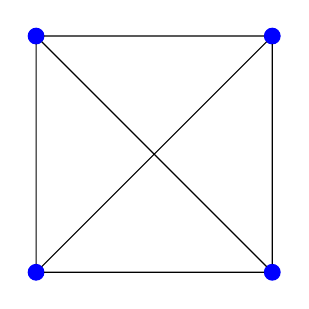
\begin{tikzpicture}[scale=0.75]
        \tikzstyle{every node}=[draw,scale=0.6,shape=circle,color=blue,fill=blue]
            \node (a) at (0,0) {};
            \node (b) at (4,0) {};
            \node (c) at (4,4) {};
            \node (d) at (0,4) {};

            \draw (a) -- (b)
            (b) -- (c)
            (a) -- (c)
            (b) -- (d)
            (a) -- (d)
            (c) -- (d);
        \end{tikzpicture}
        \end{subfigure}
        \begin{subfigure}[t]{0.4\linewidth}
        \begin{tikzpicture}[scale=0.75]
        \tikzstyle{every node}=[draw,scale=0.6,shape=circle,color=blue,fill=blue]
            \node (a) at (0,0) {};
            \node (b) at (4,0) {};
            \node (c) at (4,4) {};
            \node (d) at (0,4) {};

            \draw (a) -- (b)
            (b) -- (c)
            (b) -- (d)
            (a) -- (d)
            (c) -- (d)
            (a) edge [out=135, in=135, looseness=2] (c);
        \end{tikzpicture}
        \end{subfigure}
        \caption{The $K_4$ graph and its drawn with no crossings.}
    \end{figure}
\end{frame}

\begin{frame}{Examples}
    \begin{figure}
        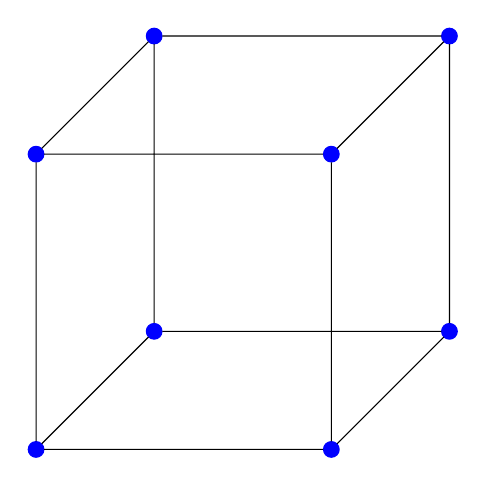
\begin{tikzpicture}[scale=0.75]
        \tikzstyle{every node}=[draw,scale=0.6,shape=circle,color=blue,fill=blue]
            \node (a) at (1,1) {};
            \node (b) at (1,6) {};
            \node (c) at (6,6) {};
            \node (d) at (6,1) {};
            \node (e) at (3,3) {};
            \node (f) at (3,8) {};
            \node (g) at (8,8) {};
            \node (h) at (8,3) {};

            \draw (a) -- (b)
            (b) -- (c)
            (c) -- (d)
            (d) -- (a)
            (e) -- (f)
            (f) -- (g)
            (g) -- (h)
            (h) -- (e)            
            (a) -- (e)
            (b) -- (f)
            (c) -- (g)
            (d) -- (h)            
            ;
        \end{tikzpicture}
        \caption{A $Q_3$ graph.}
    \end{figure}
\end{frame}

\begin{frame}{Examples}
    \begin{figure}
        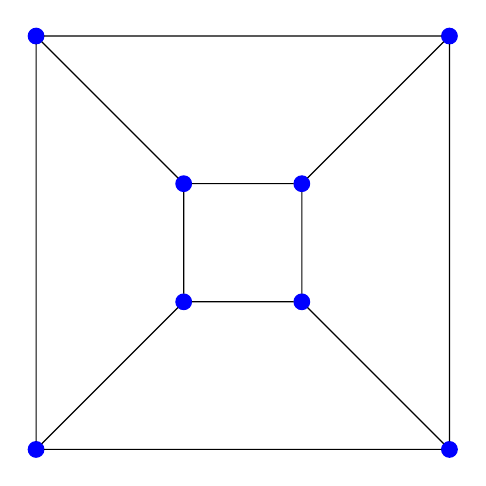
\begin{tikzpicture}[scale=0.75]
        \tikzstyle{every node}=[draw,scale=0.6,shape=circle,color=blue,fill=blue]
            \node (a) at (1,1) {};
            \node (b) at (1,8) {};
            \node (c) at (8,8) {};
            \node (d) at (8,1) {};
            \node (e) at (3.5,3.5) {};
            \node (f) at (3.5,5.5) {};
            \node (g) at (5.5,5.5) {};
            \node (h) at (5.5,3.5) {};

            \draw (a) -- (b)
            (b) -- (c)
            (c) -- (d)
            (d) -- (a)
            (e) -- (f)
            (f) -- (g)
            (g) -- (h)
            (h) -- (e)            
            (a) -- (e)
            (b) -- (f)
            (c) -- (g)
            (d) -- (h)            
            ;
        \end{tikzpicture}
        \caption{The planar representation of a $Q_3$ graph.}
    \end{figure}
\end{frame}

\begin{frame}{Euler's Formula}
    \begin{itemize}
        \item A planar representation of a graph splits the plane into regions (including an unbounded region.)
        \item Euler showed that all planar representations of a graph split the plane into the same number of regions.
        \item There is a relationship between the number of regions, vertices and edges.
    \end{itemize}
\end{frame}

\begin{frame}{Euler's Formula}
    \begin{figure}
        \begin{tikzpicture}[scale=0.75]
        \tikzstyle{every node}=[scale=0.6,shape=circle,color=blue,fill=blue]
            \node (a) at (1,1) {};
            \node (b) at (1,6) {};
            \node (c) at (6,1) {};
            \node (d) at (6,6) {};
            \node (e) at (11,1) {};
            \node (f) at (11,3.5) {};
            \node (g) at (11,6) {};
            
            \draw (a) -- (b)
            (b) -- (d)
            (d) -- (c)
            (a) -- (c)
            (b) -- (c)
            (c) -- (e)
            (d) -- (g)
            (e) -- (f)
            (f) -- (g)
            (d) -- (f)
            (c) -- (f);
            
            \node[text,scale=1.5,fill=white] at (2,2)    {$R_1$};
            \node[text,scale=1.5,fill=white] at (5,5)    {$R_2$};
            \node[text,scale=1.5,fill=white] at (7,3.5)  {$R_3$};
            \node[text,scale=1.5,fill=white] at (10,2)   {$R_4$};
            \node[text,scale=1.5,fill=white] at (10,5)   {$R_5$};
            \node[text,scale=1.5,fill=white] at (12,4) {$R_6$};
        \end{tikzpicture}
        \caption{The Regions of the Planar Representation of a Graph.}
    \end{figure}
\end{frame}

\begin{frame}{Euler's Formula}
    \begin{theorem}[EULER'S FORMULA]\label{theo:euler}
         Let $G$ be a connected planar simple graph with $e$ edges and $v$ vertices. Let $r$ be the number of regions in a planar representation of $G$. Then $r = e - v + 2$.
    \end{theorem}
\end{frame}

\section*{Reference}

\begin{frame}{Reference}
    \begin{itemize}
        \item Discrete Mathematics and Its Applications. Rosen, K.H. 2012. McGraw-Hill. \\
        \begin{itemize}
         \item Chapter 10. Graphs: \\
            Section 10.2: Graph Terminology and Special Types of Graphs. \\
            Section 10.7: Planar Graphs. 
        \end{itemize}
        \begin{itemize}
         \item Chapter 11. Trees: \\
            Section 11.1: Introduction to Trees.
        \end{itemize}
    \end{itemize}
\end{frame}

\end{document}
